% Chapter 10: Sequence Modeling: Recurrent and Recursive Nets

\chapter{Sequence Modeling: Recurrent and Recursive Nets}
\label{chap:sequence-modeling}

This chapter covers architectures designed for sequential and temporal data, including recurrent neural networks (RNNs) and their variants.


\section*{Learning Objectives}
\label{sec:ch10-learning-objectives}

After completing this chapter, you will be able to:

\begin{enumerate}
    \item \textbf{Explain why sequence models are needed} and identify data modalities that require temporal context.
    \item \textbf{Describe and compare} vanilla RNNs, LSTMs, and GRUs, including their gating mechanisms and trade-offs.
    \item \textbf{Implement and reason about} backpropagation through time (BPTT) and truncated BPTT, including gradient clipping.
    \item \textbf{Build sequence-to-sequence models with attention} and explain the intuition behind alignment and context vectors.
    \item \textbf{Apply advanced decoding and architecture variants} such as bidirectional RNNs, teacher forcing, and beam search.
    \item \textbf{Evaluate common failure modes} (vanishing/exploding gradients, exposure bias) and mitigation strategies.
\end{enumerate}




% Chapter 10, Section 1

\section{Recurrent Neural Networks \difficultyInline{intermediate}}
\label{sec:rnns}

\subsection*{Intuition}

An RNN carries a running summary of the past—like a notepad you update after reading each word. This hidden state lets the model use prior context to influence current predictions. However, keeping reliable notes over long spans is hard: small errors can compound, and gradients may shrink or grow too much \cite{GoodfellowEtAl2016}.

% \subsection*{Historical Context}

% Early sequence models struggled with long-term dependencies due to vanishing gradients, motivating gated designs such as LSTM \cite{Hochreiter1997}. Practical training stabilized with techniques like gradient clipping and better initialization \cite{GoodfellowEtAl2016}.

% Index and glossary
\index{recurrent neural network}
\glsadd{recurrent-neural-network}

\subsection{Motivation}

Sequential data exhibits \emph{temporal dependencies} and \emph{order-sensitive} structure that cannot be modeled well by i.i.d. assumptions or fixed-size context windows alone \cite{GoodfellowEtAl2016,Prince2023,Bishop2006}. Consider the diverse nature of sequential data: time series forecasting energy load, financial returns, or physiological signals like ECG readings; natural language where the meaning of a word depends entirely on its context and sentences must conform to syntax and discourse structure; speech and audio where phonemes combine to form words and coarticulation effects span multiple frames; video where actions unfold over time and temporal cues disambiguate similar frames; and control and reinforcement learning where actions influence future observations, requiring persistent memory.

Classic feedforward networks assume fixed-size inputs and lack a persistent state, making them ill-suited for long-range dependencies. Recurrent architectures introduce a hidden state that acts as a compact, learned memory \index{memory!neural} and enables conditioning on arbitrary-length histories. Historically, recurrent ideas trace back to early neural sequence models and dynamical systems; practical training matured with BPTT \cite{Rumelhart1986} and later with gated units to mitigate vanishing/exploding gradients \cite{Hochreiter1997}. For further background see the RNN overview in \cite{GoodfellowEtAl2016} and educational treatments in \cite{D2LChapterRNN,WebRNNWikipedia,WebDLBRNN}.

\index{sequence modeling}\index{temporal dependency}\glsadd{recurrent-neural-network}

\subsection{Why Sequences Matter}

The unique value of sequence modeling lies in its ability to understand how earlier elements affect later ones through context awareness, enabling the model to capture the rich dependencies that exist in temporal data. Unlike traditional approaches that treat each input independently, sequence models can work with inputs of any length, automatically adapting to the complexity and duration of the input sequence. This temporal pattern recognition capability allows the model to capture how things change over time, whether it's the evolution of language meaning, the progression of musical notes, or the development of market trends. Most importantly, this temporal understanding enables natural interaction with machines, allowing human-like communication where the system can maintain context across extended conversations and respond appropriately to the full history of the interaction.

\subsection{Basic RNN Architecture}

An RNN maintains a hidden state $\vect{h}_t$ that evolves over time:

\begin{align}
\vect{h}_t &= \sigma(\mat{W}_{hh} \vect{h}_{t-1} + \mat{W}_{xh} \vect{x}_t + \vect{b}_h) \\
\vect{y}_t &= \mat{W}_{hy} \vect{h}_t + \vect{b}_y
\end{align}

where $\vect{x}_t$ is input at time $t$, and $\sigma$ is typically tanh.

\paragraph{Visual aid.} The following unrolled diagram shows shared parameters across time:
\begin{figure}[h]
    \centering
    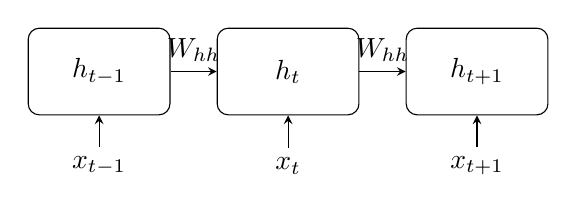
\begin{tikzpicture}[>=stealth, node distance=2.4cm]
        \tikzstyle{node}=[draw, rounded corners, minimum width=1.8cm, minimum height=1.1cm]
        \node[node] (h0) {$\vect{h}_{t-1}$};
        \node[node, right of=h0] (h1) {$\vect{h}_{t}$};
        \node[node, right of=h1] (h2) {$\vect{h}_{t+1}$};
        \draw[->] (h0) -- (h1) node[midway, above] {$\mat{W}_{hh}$};
        \draw[->] (h1) -- (h2) node[midway, above] {$\mat{W}_{hh}$};
        \node[below of=h0, yshift=1.2cm] (x0) {$\vect{x}_{t-1}$};
        \node[below of=h1, yshift=1.2cm] (x1) {$\vect{x}_{t}$};
        \node[below of=h2, yshift=1.2cm] (x2) {$\vect{x}_{t+1}$};
        \draw[->] (x0) -- (h0);
        \draw[->] (x1) -- (h1);
        \draw[->] (x2) -- (h2);
    \end{tikzpicture}
    \caption{Unrolled RNN with shared parameters across time steps.}
\end{figure}

\subsection{Unfolding in Time}

RNNs can be "unrolled" into a deep feedforward computation graph over time with \emph{shared parameters}. This perspective clarifies how gradients flow backward through temporal connections and why depth-in-time can cause vanishing/exploding gradients \cite{GoodfellowEtAl2016}.

\begin{equation}
\vect{h}_t = f(\vect{h}_{t-1}, \vect{x}_t; \vect{\theta})
\end{equation}

% \paragraph{Visual aid.} 
Unfolding reveals repeated applications of the same transition function across steps. We annotate inputs, hidden states, and outputs to emphasize sharing and the temporal chain rule during BPTT.
\begin{figure}[h]
    \centering
    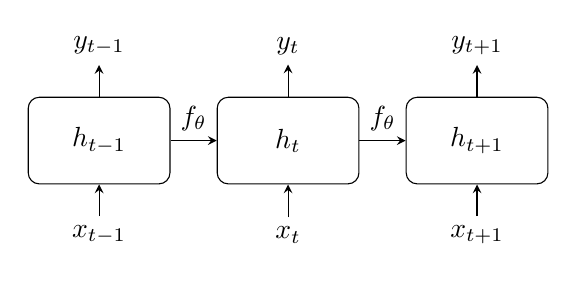
\begin{tikzpicture}[>=stealth, node distance=2.4cm]
        \tikzstyle{node}=[draw, rounded corners, minimum width=1.8cm, minimum height=1.1cm]
        \node[node] (h0) {$\vect{h}_{t-1}$};
        \node[node, right of=h0] (h1) {$\vect{h}_{t}$};
        \node[node, right of=h1] (h2) {$\vect{h}_{t+1}$};
        \draw[->] (h0) -- (h1) node[midway, above] {$f_{\vect{\theta}}$};
        \draw[->] (h1) -- (h2) node[midway, above] {$f_{\vect{\theta}}$};
        \node[below of=h0, yshift=1.2cm] (x0) {$\vect{x}_{t-1}$};
        \node[below of=h1, yshift=1.2cm] (x1) {$\vect{x}_{t}$};
        \node[below of=h2, yshift=1.2cm] (x2) {$\vect{x}_{t+1}$};
        \draw[->] (x0) -- (h0);
        \draw[->] (x1) -- (h1);
        \draw[->] (x2) -- (h2);
        \node[above of=h0, yshift=-1.2cm] (y0) {$\vect{y}_{t-1}$};
        \node[above of=h1, yshift=-1.2cm] (y1) {$\vect{y}_{t}$};
        \node[above of=h2, yshift=-1.2cm] (y2) {$\vect{y}_{t+1}$};
        \draw[->] (h0) -- (y0);
        \draw[->] (h1) -- (y1);
        \draw[->] (h2) -- (y2);
    \end{tikzpicture}
    \caption{Unrolling an RNN across time: the same parameters $\vect{\theta}$ are reused at each step.}
\end{figure}

This view connects RNNs to dynamic Bayesian networks and emphasizes that training complexity scales with the unroll length. See \cite{WebRNNWikipedia,GoodfellowEtAl2016,D2LChapterRNN}.

\index{unrolling in time}\index{shared parameters}

\subsection{Types of Sequences}

\begin{table}[h]
\centering
\begin{tabularx}{0.9\textwidth}{p{0.15\textwidth} *{2}{X}}
\toprule
\textbf{Type} & \textbf{Description} & \textbf{Examples} \\
\midrule
One-to-one & Fixed-size input to fixed-size output with temporal structure ignored or not present & Static image classification \\
\midrule
One-to-many & Single input to sequence output & Image captioning \\
\midrule
Many-to-one & Sequence input to single output & Sentiment classification; keyword spotting \\
\midrule
Many-to-many (synchronous) & Sequence labeling with aligned input/output lengths & Part-of-speech tagging; frame labeling \\
\midrule
Many-to-many (asynchronous) & Sequence transduction with potentially different lengths. Attention helps bridge length mismatch by learning soft alignments \cite{Bahdanau2014} & Machine translation; speech recognition \\
\bottomrule
\end{tabularx}
\caption{Types of sequence models and their characteristics.}
\label{tab:sequence-types}
\end{table}

Design choices (teacher forcing, bidirectionality, attention, beam search) depend on whether future context is available and whether output timing must be causal. See \cite{D2LChapterRNN,WebRNNWikipedia} for further taxonomy.

\index{sequence types}\index{sequence labeling}\index{sequence transduction}

% Citations
See \cite{GoodfellowEtAl2016,Prince2023,Bishop2006,WebRNNWikipedia,WebDLBRNN,D2LChapterRNN} for introductions to sequence modeling and RNNs.


% Chapter 10, Section 2

\section{Backpropagation Through Time \difficultyInline{intermediate}}
\label{sec:bptt}

\subsection*{Intuition}

BPTT treats the unrolled RNN as a deep network across time and applies backpropagation through each time slice. Gradients flow backward along temporal edges, accumulating effects from future steps. Truncation limits how far signals propagate to balance cost and dependency length \cite{GoodfellowEtAl2016}.

\subsection*{Historical Context}

The backpropagation algorithm \cite{Rumelhart1986} enabled efficient training of deep networks; applying it to unrolled RNNs became known as BPTT. Awareness of vanishing/exploding gradients led to clipping and gated architectures \cite{GoodfellowEtAl2016,Hochreiter1997}.

% Index and glossary
\index{backpropagation through time}
\glsadd{vanishing-gradient}
\glsadd{exploding-gradient}

\subsection{BPTT Algorithm}

Gradients are computed by unrolling the network and applying backpropagation through the temporal graph. Let $L=\sum_{t=1}^{T} L_t$ and $\vect{h}_t = f(\vect{h}_{t-1}, \vect{x}_t; \vect{\theta})$, $\vect{y}_t = g(\vect{h}_t; \vect{\theta}_y)$. The total derivative w.r.t. hidden states satisfies the recurrence:

\begin{equation}
\frac{\partial L}{\partial \vect{h}_t} = \frac{\partial L}{\partial \vect{y}_t} \frac{\partial \vect{y}_t}{\partial \vect{h}_t} + \frac{\partial L}{\partial \vect{h}_{t+1}} \frac{\partial \vect{h}_{t+1}}{\partial \vect{h}_t}
\end{equation}

For any parameter block $\mat{W} \in \vect{\theta}$ appearing at each time step:
\begin{equation}
\frac{\partial L}{\partial \mat{W}} = \sum_{t=1}^{T} \frac{\partial L_t}{\partial \mat{W}}
\end{equation}

\paragraph{Algorithm (BPTT).}
\begin{enumerate}[nosep]
    \item Forward pass: for $t=1,\dots,T$, compute $\vect{h}_t$, $\vect{y}_t$, and $L_t$.
    \item Initialize temporal gradients: $\frac{\partial L}{\partial \vect{h}_{T+1}}=\vect{0}$.
    \item Backward pass: for $t=T,\dots,1$:
    \begin{align*}
        \delta_t &\leftarrow \frac{\partial L}{\partial \vect{y}_t} \frac{\partial \vect{y}_t}{\partial \vect{h}_t} + \left(\frac{\partial L}{\partial \vect{h}_{t+1}}\right) \frac{\partial \vect{h}_{t+1}}{\partial \vect{h}_t} \\
        \frac{\partial L}{\partial \mat{W}} &\mathrel{+}= \delta_t \frac{\partial \vect{h}_t}{\partial \mat{W}} \quad (\text{or add contributions for all parameters at time } t)
    \end{align*}
    \item Apply gradient clipping if needed and update parameters.
\end{enumerate}

This view aligns with the computational-graph treatment in \cite{GoodfellowEtAl2016} and standard expositions \cite{WebDLBRNN,D2LChapterRNN}.

\subsection{Vanishing and Exploding Gradients}

Gradients can vanish or explode exponentially:

\begin{equation}
\frac{\partial \vect{h}_t}{\partial \vect{h}_k} = \prod_{i=k+1}^{t} \frac{\partial \vect{h}_i}{\partial \vect{h}_{i-1}} = \prod_{i=k+1}^{t} \mat{W}^\top \text{diag}(\sigma'(\vect{z}_i))
\end{equation}

If eigenvalues of $\mat{W}$ are:
\begin{itemize}
    \item $< 1$: gradients vanish
    \item $> 1$: gradients explode
\end{itemize}

\textbf{Solutions:}
\begin{itemize}
    \item Gradient clipping (for explosion) \glsadd{gradient-clipping}
    \item Careful initialization
    \item ReLU activation
    \item LSTM/GRU architectures
\end{itemize}

\subsection{Truncated BPTT}

For very long sequences, truncate gradient computation by limiting backpropagation to a sliding window of $k$ steps \cite{GoodfellowEtAl2016}:
\begin{itemize}
    \item Process inputs in segments of length $k$ (possibly overlapping with stride $s$).
    \item Backpropagate gradients only within each segment to reduce memory and time.
    \item Hidden state is carried forward between segments but treated as a constant during the truncated backward step.
\end{itemize}

\paragraph{Algorithm (Truncated BPTT).}
\begin{enumerate}[nosep]
    \item For $t=1,1+s,1+2s,\dots$, take the chunk $[t,\, t+k-1]$.
    \item Run forward pass over the chunk using the current hidden state as initialization.
    \item Backpropagate losses only within the chunk; accumulate gradients.
    \item Optionally detach the final hidden state from the graph before the next chunk to bound gradient length.
\end{enumerate}

\textbf{Trade-offs:} Lower memory and latency versus potentially missing very long-range dependencies. Increasing $k$ improves dependency length coverage but increases cost. Hybrids with dilated RNNs or attention can mitigate the trade-off.


% Chapter 10, Section 3

\section{Long Short-Term Memory (LSTM) \difficultyInline{intermediate}}
\label{sec:lstm}

\subsection*{Intuition}

The LSTM adds a highway for information (the cell state) that can pass signals forward with minimal modification. Gates act like valves to forget unhelpful information, write new content, and reveal outputs, which preserves gradients over long spans \cite{Hochreiter1997,GoodfellowEtAl2016}.

\subsection*{Historical Context}

Introduced in the 1990s to address vanishing gradients \cite{Hochreiter1997}, LSTMs unlocked practical sequence learning across speech, language, and time-series tasks before attention-based Transformers became dominant \cite{Vaswani2017}.

% Index and glossary
\index{long short-term memory}
\glsadd{long-short-term-memory}

\subsection{Architecture}

LSTM uses \textbf{gating mechanisms} to control information flow and maintain a persistent cell state that supports long-range credit assignment \cite{Hochreiter1997,GoodfellowEtAl2016}. Let $\vect{h}_{t-1} \in \mathbb{R}^h$ denote the hidden state from the previous time step, $\vect{x}_t \in \mathbb{R}^d$ the current input, and $\vect{c}_{t-1} \in \mathbb{R}^h$ the previous cell state. The concatenation $[\vect{h}_{t-1}, \vect{x}_t] \in \mathbb{R}^{h+d}$ combines both sources of information. The LSTM computes the following:

\begin{align}
\vect{f}_t &= \sigma(\mat{W}_f [\vect{h}_{t-1}, \vect{x}_t] + \vect{b}_f) \quad \text{(forget gate)} \\
\vect{i}_t &= \sigma(\mat{W}_i [\vect{h}_{t-1}, \vect{x}_t] + \vect{b}_i) \quad \text{(input gate)} \\
\tilde{\vect{c}}_t &= \tanh(\mat{W}_c [\vect{h}_{t-1}, \vect{x}_t] + \vect{b}_c) \quad \text{(candidate)} \\
\vect{c}_t &= \vect{f}_t \odot \vect{c}_{t-1} + \vect{i}_t \odot \tilde{\vect{c}}_t \quad \text{(cell state)} \\
\vect{o}_t &= \sigma(\mat{W}_o [\vect{h}_{t-1}, \vect{x}_t] + \vect{b}_o) \quad \text{(output gate)} \\
\vect{h}_t &= \vect{o}_t \odot \tanh(\vect{c}_t) \quad \text{(hidden state)}
\end{align}

where $\sigma(\cdot)$ denotes the sigmoid function $\sigma(z) = 1/(1+e^{-z})$ applied element-wise, $\tanh(\cdot)$ is the hyperbolic tangent activation, and $\odot$ represents the Hadamard (element-wise) product. The weight matrices have dimensions $\mat{W}_f, \mat{W}_i, \mat{W}_c, \mat{W}_o \in \mathbb{R}^{h \times (h+d)}$ and bias vectors $\vect{b}_f, \vect{b}_i, \vect{b}_c, \vect{b}_o \in \mathbb{R}^h$.

The cell state update equation $\vect{c}_t = \vect{f}_t \odot \vect{c}_{t-1} + \vect{i}_t \odot \tilde{\vect{c}}_t$ can be understood as a gated linear interpolation. When $\vect{f}_t \approx \vect{1}$ (forget gate fully open) and $\vect{i}_t \approx \vect{0}$ (input gate closed), the cell state is preserved: $\vect{c}_t \approx \vect{c}_{t-1}$. When $\vect{f}_t \approx \vect{0}$ and $\vect{i}_t \approx \vect{1}$, the cell state is replaced: $\vect{c}_t \approx \tilde{\vect{c}}_t$. In practice, both gates take intermediate values, allowing partial forgetting and partial updating.

\subsection{Key Ideas}

The LSTM's key innovations address fundamental limitations of traditional RNNs and feedforward networks. Unlike standard RNNs where information must pass through repeated nonlinear transformations that cause gradient decay, the LSTM introduces a dedicated \textbf{cell state} $\vect{c}_t$ that acts as a highway for information flow with minimal transformation, enabling gradients to flow directly across long time spans. The \textbf{gating mechanisms} (forget, input, and output gates) provide selective control over information flow, allowing the network to learn when to remember, forget, and output information—a capability that was impossible with fixed-weight feedforward networks or vanilla RNNs. This selective memory management solves the vanishing gradient problem by creating direct paths for gradient flow while maintaining the ability to learn complex temporal dependencies that exceed the capacity of traditional sequence models.

\textbf{Cell state} $\vect{c}_t$: Long-term memory
\begin{itemize}
    \item Information flows with minimal transformation
    \item Gates control what to remember/forget
\end{itemize}

\textbf{Forget gate} $\vect{f}_t$: Decides what to discard from cell state

\textbf{Input gate} $\vect{i}_t$: Decides what new information to store

\textbf{Output gate} $\vect{o}_t$: Decides what to output

\subsection{Advantages}

\textbf{Addresses vanishing gradient problem:} LSTMs mitigate vanishing gradients through their cell state and gating mechanisms. Consider the gradient of the loss $L$ with respect to the cell state at an earlier time $k$:
\begin{equation}
\frac{\partial L}{\partial \vect{c}_k} = \frac{\partial L}{\partial \vect{c}_t} \prod_{i=k+1}^{t} \frac{\partial \vect{c}_i}{\partial \vect{c}_{i-1}}
\end{equation}
where $\frac{\partial \vect{c}_i}{\partial \vect{c}_{i-1}} = \text{diag}(\vect{f}_i)$ from the cell state update rule. When forget gates are close to 1, this product involves multiplications close to identity, preventing gradient decay. Unlike vanilla RNNs where $\frac{\partial \vect{h}_i}{\partial \vect{h}_{i-1}} = \mat{W}^\top \text{diag}(\sigma'(\vect{z}_i))$ involves repeated matrix multiplications that compound eigenvalue effects, the LSTM's cell state path provides a more direct gradient highway.

\textbf{Can learn long-term dependencies:} The forget and input gates explicitly control information retention through learnable parameters. The effective memory span can be approximated by considering when $\vect{f}_i \approx \vect{1}$ for all $i \in [k, t]$, the cell state propagates with minimal modification: $\vect{c}_t \approx \vect{c}_k + \sum_{i=k+1}^{t} \vect{i}_i \odot \tilde{\vect{c}}_i$. This additive structure, rather than multiplicative, allows information to persist over hundreds of time steps. The selective gating learns to retain task-relevant information whilst discarding noise.

\textbf{Gradients flow more easily through cell state:} The gradient flow through the cell state can be written as:
\begin{equation}
\frac{\partial L}{\partial \vect{c}_{t-1}} = \frac{\partial L}{\partial \vect{c}_t} \odot \vect{f}_t + \frac{\partial L}{\partial \vect{h}_t} \odot \vect{o}_t \odot (1 - \tanh^2(\vect{c}_t)) \odot \vect{f}_t
\end{equation}
The first term shows that when $\vect{f}_t \approx \vect{1}$, gradients pass through almost unchanged: $\frac{\partial L}{\partial \vect{c}_{t-1}} \approx \frac{\partial L}{\partial \vect{c}_t}$. This linear-like flow, especially when the forget gate is close to 1, prevents the repeated multiplication by small weights that causes gradients to vanish in vanilla RNNs where $\frac{\partial L}{\partial \vect{h}_{t-1}} \propto \mat{W}^\top \sigma'(\cdot)$. The gating mechanism creates a more stable gradient propagation environment by adaptively controlling gradient flow.

\textbf{Widely used for sequential tasks:} Due to their ability to handle long-term dependencies and mitigate gradient issues, LSTMs have become a de facto standard for various sequential data processing tasks. Their robust performance across diverse applications, from natural language processing to speech recognition, underscores their versatility and effectiveness. The architecture's success has made it a go-to choice for practitioners working with temporal data.

\begin{figure}[h]
    \centering
    \begin{tikzpicture}[>=stealth, node distance=1.8cm]
        \tikzstyle{gate}=[draw, rounded corners, minimum width=1.5cm, minimum height=0.9cm]
        \node[gate] (ft) {$\vect{f}_t$};
        \node[gate, below of=ft] (it) {$\vect{i}_t$};
        \node[gate, below of=it] (ot) {$\vect{o}_t$};
        \node[right of=it, xshift=2.2cm] (ct1) {$\vect{c}_{t-1}$};
        \node[right of=ct1, xshift=1.2cm] (sum) {$+$};
        \node[right of=sum, xshift=1.2cm] (ct) {$\vect{c}_t$};
        \draw[->] (ct1) -- node[midway, above] {$\odot\,\vect{f}_t$} (sum);
        \draw[->] (it) -- node[midway, above] {$\odot\,\tilde{\vect{c}}_t$} (sum);
        \draw[->] (sum) -- (ct);
        \draw[->] (ot) |- ++(1.2,1.8) node[pos=0.55, right] {$\odot\,\tanh(\vect{c}_t)$} -| ++(0,0);
    \end{tikzpicture}
    \caption{Visual aid: A compact LSTM cell diagram.}
    \label{fig:lstm_cell_diagram}
\end{figure}


% Chapter 10, Section 4

\section{Gated Recurrent Units (GRU) \difficultyInline{intermediate}}
\label{sec:gru}

\subsection*{Intuition}

GRU simplifies LSTM by merging cell and hidden state and combining gates, often matching performance with fewer parameters—useful when data or compute is limited \cite{Cho2014,GoodfellowEtAl2016}.

\subsection*{Historical Context}

Proposed in the mid-2010s, GRU offered a practical alternative to LSTM with competitive empirical results and simpler implementation \cite{Cho2014}.

% Index and glossary
\index{gated recurrent unit}
\glsadd{recurrent-neural-network}

\subsection{Architecture}

GRU simplifies LSTM with fewer parameters and merges the cell and hidden state into a single vector, often yielding comparable performance with less computation \cite{Cho2014,GoodfellowEtAl2016}:

\begin{align}
\vect{z}_t &= \sigma(\mat{W}_z [\vect{h}_{t-1}, \vect{x}_t]) \quad \text{(update gate)} \\
\vect{r}_t &= \sigma(\mat{W}_r [\vect{h}_{t-1}, \vect{x}_t]) \quad \text{(reset gate)} \\
\tilde{\vect{h}}_t &= \tanh(\mat{W} [\vect{r}_t \odot \vect{h}_{t-1}, \vect{x}_t]) \quad \text{(candidate)} \\
\vect{h}_t &= (1 - \vect{z}_t) \odot \vect{h}_{t-1} + \vect{z}_t \odot \tilde{\vect{h}}_t
\end{align}

\subsection{Architecture (visual)}
\begin{figure}[h]
    \centering
    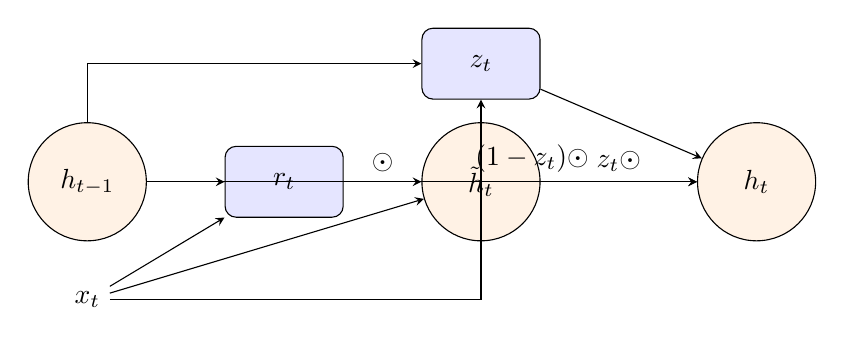
\begin{tikzpicture}[>=stealth, node distance=2.0cm]
        \tikzstyle{gate}=[draw, rounded corners, minimum width=1.5cm, minimum height=0.9cm, fill=blue!10]
        \tikzstyle{state}=[draw, circle, minimum width=1.5cm, fill=orange!10]
        
        % Previous hidden state
        \node[state] (ht1) {$\vect{h}_{t-1}$};
        
        % Input
        \node[below of=ht1, yshift=0.5cm] (xt) {$\vect{x}_t$};
        
        % Reset gate
        \node[gate, right of=ht1, xshift=0.5cm] (rt) {$\vect{r}_t$};
        
        % Candidate hidden state
        \node[state, right of=rt, xshift=0.5cm] (cand) {$\tilde{\vect{h}}_t$};
        
        % Update gate
        \node[gate, above of=cand, yshift=-0.5cm] (zt) {$\vect{z}_t$};
        
        % Current hidden state
        \node[state, right of=cand, xshift=1.5cm] (ht) {$\vect{h}_t$};
        
        % Arrows
        \draw[->] (ht1) -- (rt);
        \draw[->] (xt) -- (rt);
        \draw[->] (xt) -| (zt);
        \draw[->] (ht1) |- (zt);
        \draw[->] (rt) -- node[midway, above] {$\odot$} (cand);
        \draw[->] (xt) -- (cand);
        \draw[->] (cand) -- node[midway, above] {$\vect{z}_t \odot$} (ht);
        \draw[->] (ht1) -- node[pos=0.7, above] {$(1-\vect{z}_t) \odot$} (ht);
        \draw[->] (zt) -- (ht);
    \end{tikzpicture}
    \caption{GRU architecture showing update gate $\vect{z}_t$, reset gate $\vect{r}_t$, and information flow from $\vect{h}_{t-1}$ and $\vect{x}_t$ to $\vect{h}_t$.}
    \label{fig:gru_architecture}
\end{figure}

\subsection{Comparison with LSTM}
\begin{table}[h]
    \centering
    \begin{tabular}{@{}p{3.2cm}p{5.2cm}p{5.2cm}@{}}
    \toprule
    & \textbf{GRU} & \textbf{LSTM} \\
    \midrule
    State & Single hidden state $\vect{h}_t$ & Hidden $\vect{h}_t$ and cell $\vect{c}_t$ \\
    Gates & Update, reset & Input, forget, output \\
    Parameters & Fewer (often faster) & More (more expressive) \\
    Long-range deps. & Good in practice & Often stronger on very long spans \\
    Simplicity & Simpler to implement & Slightly more complex \\
    Typical use & Smaller data/compute budgets & Longer sequences or when capacity helps \\
    \bottomrule
    \end{tabular}
    \caption{GRU vs. LSTM at a glance \cite{Cho2014,Hochreiter1997,GoodfellowEtAl2016}.}
\end{table}

The choice between GRU and LSTM often depends on the specific task requirements and computational constraints. GRU's simpler architecture with fewer parameters makes it computationally more efficient, typically requiring less memory and allowing for faster training, which can be particularly advantageous when working with limited computational resources or when rapid prototyping is needed. Empirically, GRU performance is often comparable to LSTM on many tasks, especially those with moderate sequence lengths, though LSTM tends to have a slight edge on problems requiring very long-term dependencies due to its separate cell state that can maintain information more independently. In practice, both architectures have proven highly effective, and the choice often comes down to experimentation—trying both on your specific dataset and choosing the one that yields better validation performance whilst considering training time and deployment constraints. Modern deep learning frameworks make it straightforward to swap between these architectures, so practitioners can easily evaluate both options during model development.


% Chapter 10, Section 5

\section{Sequence-to-Sequence Models \difficultyInline{intermediate}}
\label{sec:seq2seq}

\subsection*{Intuition}

Encoder–decoder models compress a source sequence into a representation and then generate a target sequence step-by-step. Attention augments this by letting the decoder look back at encoder states as needed, creating a dynamic context per output token \cite{Cho2014,Bahdanau2014}.

% \subsection*{Historical Context}

% Early seq2seq relied on fixed context vectors, which degraded on long inputs. Content-based attention \cite{Bahdanau2014} lifted this bottleneck and paved the way toward Transformer architectures \cite{Vaswani2017}.

% Index and glossary
\index{sequence-to-sequence}
\glsadd{attention-mechanism}

\subsection{Encoder-Decoder Architecture}

The encoder-decoder architecture revolutionized sequence-to-sequence learning by solving a fundamental challenge: how to transform variable-length input sequences into variable-length output sequences of potentially different lengths. Traditional approaches struggled with this asymmetry, as they required fixed input-output dimensions or relied on hand-crafted features that couldn't capture the complex relationships between source and target sequences. The key insight behind this architecture lies in its elegant separation of concerns: the encoder compresses the entire input sequence into a rich, fixed-size representation that captures all essential information, while the decoder uses this representation to generate the output sequence step-by-step, maintaining the temporal dependencies crucial for coherent generation. This design was revolutionary compared to previous architectures because it eliminated the need for explicit alignment between input and output positions, allowing the model to learn implicit correspondences through end-to-end training. Unlike rule-based systems or traditional statistical methods that required extensive linguistic knowledge, the encoder-decoder framework could automatically discover complex mappings between any two sequence domains, making it the foundation for modern neural machine translation and countless other sequence transduction tasks.

For sequence transduction tasks like machine translation \cite{Cho2014,Bahdanau2014}:

\textbf{Encoder:} Processes input sequence into representation (fixed or per-step states)
\begin{equation}
\vect{c} = f(\vect{x}_1, \vect{x}_2, \ldots, \vect{x}_T)
\end{equation}

\textbf{Decoder:} Generates output sequence from representation

% \paragraph{Visual aid.} 

A minimal encoder–decoder with context vector.
\begin{figure}[h]
    \centering
    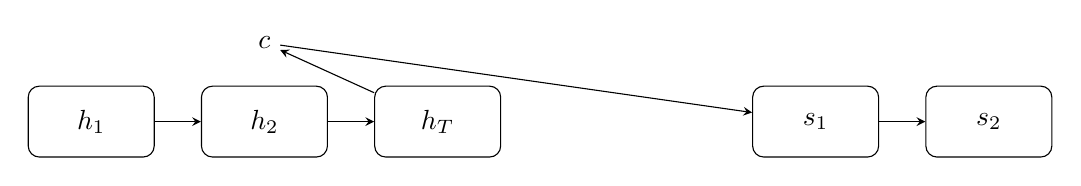
\begin{tikzpicture}[>=stealth, node distance=2.2cm]
        \tikzstyle{enc}=[draw, rounded corners, minimum width=1.6cm, minimum height=0.9cm]
        \tikzstyle{dec}=[draw, rounded corners, minimum width=1.6cm, minimum height=0.9cm]
        \node[enc] (e1) {$\vect{h}_1$};
        \node[enc, right of=e1] (e2) {$\vect{h}_2$};
        \node[enc, right of=e2] (eT) {$\vect{h}_T$};
        \node[above of=e2, yshift=-1.2cm] (c) {$\vect{c}$};
        \draw[->] (e1) -- (e2);
        \draw[->] (e2) -- (eT);
        \draw[->] (eT) -- (c);
        \node[dec, right of=eT, xshift=2.6cm] (d1) {$\vect{s}_1$};
        \node[dec, right of=d1] (d2) {$\vect{s}_2$};
        \draw[->] (c) -- (d1);
        \draw[->] (d1) -- (d2);
    \end{tikzpicture}
    \caption{Encoder–decoder with fixed context vector $\vect{c}$. Attention uses step-dependent $\vect{c}_t$.}
\end{figure}

\begin{equation}
\vect{y}_t = g(\vect{y}_{t-1}, \vect{c}, \vect{s}_{t-1})
\end{equation}

\subsection{Attention Mechanism: Attention Is All You Need}

Attention represents one of the most crucial breakthroughs in deep learning, so fundamental that the seminal paper "Attention Is All You Need" \cite{Vaswani2017} demonstrated that attention mechanisms alone could replace entire architectural components like recurrent layers. This paradigm shift occurred because attention solves the fundamental information bottleneck problem in sequence-to-sequence models, where standard approaches compress entire input sequences into a single fixed vector $\vect{c}$, inevitably losing critical information and context. The attention mechanism elegantly addresses this limitation by allowing the decoder to dynamically focus on different parts of the input sequence at each generation step, creating a flexible and context-aware representation that adapts to the specific requirements of each output token.

\textbf{Attention} allows the decoder to focus on relevant input parts by computing a content-based weighted average of encoder states \cite{Bahdanau2014}. At each decoding step $t$:

\begin{align}
e_{ti} &= a(\vect{s}_{t-1}, \vect{h}_i) \quad \text{(alignment scores)} \\
\alpha_{ti} &= \frac{\exp(e_{ti})}{\sum_j \exp(e_{tj})} \quad \text{(attention weights)} \\
\vect{c}_t &= \sum_i \alpha_{ti} \vect{h}_i \quad \text{(context vector)}
\end{align}
Common scoring functions $a(\cdot)$ include additive (Bahdanau) attention using a small MLP, and multiplicative/dot-product attention which is parameter-efficient and forms the basis for scaled dot-product attention in Transformers \cite{Vaswani2017}. Attention weights $\alpha_{ti}$ are interpretable as soft alignments between target position $t$ and source position $i$ (see \cite{WebAttentionWikipedia}). For a broader overview, consult standard references \cite{WebDLBRNN,D2LChapterAttention}.

\paragraph{Training and inference.} Attention is trained end-to-end with the seq2seq objective. During inference, attention enables the model to retrieve the most relevant encoder features for each generated token, improving long-input performance and handling reordering. Variants include multi-head attention, local/monotonic attention for streaming, and coverage terms to reduce repetition.

% Benefits:

\textbf{Dynamic context for each output:} Unlike traditional approaches that use a single, static context vector for all output positions, attention creates a unique, dynamically computed context vector for each decoding step. This means that when generating the word "cat" in a translation, the model can focus on the relevant source words like "gato" or "chat," while when generating "dog," it shifts its attention to "perro" or "chien." This adaptive context selection allows the model to maintain fine-grained relationships between source and target elements, dramatically improving translation quality and coherence across different linguistic structures.

\textbf{Better for long sequences:} Traditional encoder-decoder models suffer from severe performance degradation on long sequences because the fixed-size context vector becomes an information bottleneck, unable to preserve all the nuanced details from lengthy inputs. Attention mechanisms solve this by providing direct access to all encoder states, allowing the model to selectively retrieve relevant information regardless of sequence length. This capability is particularly crucial for tasks like document summarization or translating lengthy articles, where the model must maintain awareness of information from the beginning of the document even when generating the final sentences.

\textbf{Interpretable (visualize attention weights):} One of the most remarkable aspects of attention mechanisms is their inherent interpretability, as the attention weights $\alpha_{ti}$ provide a clear, visual representation of which input positions the model considers most relevant for each output token. Researchers can visualize these attention patterns as heatmaps, revealing fascinating insights about how the model learns linguistic alignments, syntactic structures, and semantic relationships. This interpretability has proven invaluable for debugging model behavior, understanding translation errors, and even discovering novel linguistic patterns that the model has learned autonomously, making attention not just a powerful computational tool but also a window into the model's decision-making process.

\subsection{Applications}

\textbf{Machine translation (NMT):} Modern neural machine translation systems power real-time communication across language barriers, enabling instant translation of web pages, documents, and conversations in applications like Google Translate and Microsoft Translator. These systems handle complex linguistic phenomena such as idiomatic expressions, cultural references, and context-dependent meanings that traditional rule-based systems struggled with, making global communication seamless for billions of users worldwide.

\textbf{Text summarization (extractive and abstractive):} News organizations and content platforms rely on sequence-to-sequence models to automatically generate concise summaries of lengthy articles, research papers, and legal documents, helping readers quickly grasp key information without reading entire texts. Financial institutions use these systems to summarize market reports and regulatory documents, while healthcare organizations employ them to distill complex medical literature into actionable insights for practitioners.

\textbf{Question answering and dialogue systems:} Virtual assistants like Siri, Alexa, and Google Assistant leverage sequence-to-sequence architectures to understand user queries and generate natural, contextually appropriate responses across diverse topics and conversation styles. Customer service chatbots powered by these models can handle complex inquiries, maintain conversation context across multiple turns, and provide personalized assistance while reducing human workload and improving response times.

\textbf{Image captioning (CNN/ViT encoder, RNN/Transformer decoder):} Social media platforms and accessibility tools use image captioning to automatically generate descriptive text for photos, helping visually impaired users understand visual content and improving content discoverability through search. Medical imaging systems employ these models to generate detailed reports from X-rays and MRI scans, while autonomous vehicles use them to describe road conditions and potential hazards for safety systems.

\textbf{Speech recognition and speech translation:} Real-time meeting transcription services like Otter.ai and Zoom's live transcription feature use sequence-to-sequence models to convert spoken language into accurate text, enabling accessibility and note-taking for millions of users. Simultaneous interpretation systems at international conferences and diplomatic meetings leverage these technologies to provide real-time translation between speakers of different languages, breaking down communication barriers in global settings.

\textbf{OCR and handwriting recognition:} Banking and financial institutions use OCR systems to automatically process handwritten checks, forms, and documents, dramatically reducing manual data entry and processing time while minimizing human errors. Educational platforms employ handwriting recognition to digitize student notes and assignments, enabling digital archiving, search, and analysis of handwritten content across academic institutions.

\textbf{Code generation and program repair:} Software development platforms like GitHub Copilot and Tabnine use sequence-to-sequence models to suggest code completions, generate functions from natural language descriptions, and automatically fix bugs in existing codebases. These systems help developers write code faster, catch potential errors early, and learn new programming patterns, while automated program repair tools can identify and fix security vulnerabilities and performance issues in large-scale software projects.


% Chapter 10, Section 6

\section{Advanced Topics \difficultyInline{intermediate}}
\label{sec:rnn-advanced}

\subsection*{Intuition}

Variants extend context (bidirectional), depth (stacked layers), supervision signals (teacher forcing), and search quality (beam search). Beam search maintains multiple candidate sequences during generation, exploring promising paths rather than committing to a single greedy choice, which often leads to higher-quality outputs. These architectural and algorithmic choices create fundamental trade-offs that practitioners must navigate carefully. Training stability often comes at the cost of inference complexity, while improved context modeling may increase computational requirements. The optimal configuration depends heavily on the specific task requirements, available computational resources, and latency constraints. For example, real-time applications may prioritize speed over quality, while offline processing can afford more sophisticated search strategies. Understanding these trade-offs is crucial for designing effective RNN-based systems that meet both performance and practical deployment requirements.

\subsection*{Historical Context}

Bidirectional RNNs (BiRNN) emerged post-2000 as a key innovation to improve context use for labeling tasks like Part-of-Speech tagging. Instead of processing sequences unidirectionally, BiRNNs use two independent RNNs (often LSTMs): one running forward and one backward, with their outputs concatenated. This structure allows any element $x_t$ to benefit from both past and future context, resulting in much richer local context for classification. Teacher forcing stabilized decoder training but highlighted exposure bias; beam search became standard for autoregressive decoding in translation and speech.

% Index and glossary
\index{bidirectional RNN}
\index{teacher forcing}
\index{beam search}
\glsadd{attention-mechanism}

\subsection{Bidirectional RNNs}

The term "bidirectional" refers to processing the input sequence in both temporal directions—forward and backward—unlike standard RNNs that only process left-to-right. Mathematically, this means maintaining two separate hidden state sequences:

\begin{align}
\overrightarrow{\vect{h}}_t &= f(\vect{x}_t, \overrightarrow{\vect{h}}_{t-1}) \\
\overleftarrow{\vect{h}}_t &= f(\vect{x}_t, \overleftarrow{\vect{h}}_{t+1}) \\
\vect{h}_t &= [\overrightarrow{\vect{h}}_t; \overleftarrow{\vect{h}}_t]
\end{align}

The forward arrow $\overrightarrow{\vect{h}}_t$ processes the sequence from left to right (time $t-1$ to $t$), while the backward arrow $\overleftarrow{\vect{h}}_t$ processes from right to left (time $t+1$ to $t$). The final representation $\vect{h}_t$ concatenates both directions, giving each position access to both past and future context.

\paragraph{Metaphor.} Imagine reading a sentence twice: first normally from left to right to understand the flow, then reading it backward from right to left to catch any nuances you might have missed. A bidirectional RNN does exactly this—it "reads" the sequence in both directions simultaneously, allowing each word to be understood in the full context of what comes before and after it.

Useful when future context is available.

\paragraph{Use cases and caveats.} Effective for tagging, chunking, and ASR with full utterances, but not suitable for strictly causal, low-latency streaming since backward states require future tokens. Alternatives include limited-lookahead or online approximations.

\subsection{Deep RNNs}

Stack multiple RNN layers:
\begin{equation}
\vect{h}_t^{(l)} = f(\vect{h}_t^{(l-1)}, \vect{h}_{t-1}^{(l)})
\end{equation}

The term "deep" refers to the vertical stacking of multiple recurrent layers, where each layer $l$ processes the hidden states from the previous layer $l-1$ at each time step. This creates a hierarchical representation where lower layers capture local patterns and dependencies, while higher layers learn more complex, long-range temporal relationships. Unlike feedforward networks where depth refers to the number of layers, in deep RNNs, depth combines both the number of layers and the temporal dimension, creating a two-dimensional computational graph. Each layer can specialize in different aspects of the sequence modeling task, with early layers often focusing on local features and later layers integrating information across longer time horizons.

\paragraph{Visual aid.} Stacked recurrent layers over time.
\begin{figure}[h]
    \centering
    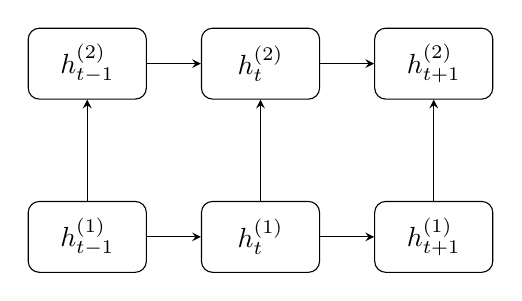
\begin{tikzpicture}[>=stealth, node distance=2.2cm]
        \tikzstyle{node}=[draw, rounded corners, minimum width=1.5cm, minimum height=0.9cm]
        % time t-1
        \node[node] (l1t1) {$\vect{h}_{t-1}^{(1)}$};
        \node[node, above of=l1t1] (l2t1) {$\vect{h}_{t-1}^{(2)}$};
        % time t
        \node[node, right of=l1t1] (l1t) {$\vect{h}_{t}^{(1)}$};
        \node[node, above of=l1t] (l2t) {$\vect{h}_{t}^{(2)}$};
        % time t+1
        \node[node, right of=l1t] (l1t2) {$\vect{h}_{t+1}^{(1)}$};
        \node[node, above of=l1t2] (l2t2) {$\vect{h}_{t+1}^{(2)}$};
        % horizontal
        \draw[->] (l1t1) -- (l1t);
        \draw[->] (l1t) -- (l1t2);
        \draw[->] (l2t1) -- (l2t);
        \draw[->] (l2t) -- (l2t2);
        % vertical
        \draw[->] (l1t1) -- (l2t1);
        \draw[->] (l1t) -- (l2t);
        \draw[->] (l1t2) -- (l2t2);
    \end{tikzpicture}
    \caption{Deep RNN: multiple recurrent layers stacked over time.}
\end{figure}

Practical tips: residual connections, layer normalization, and dropout between layers help optimization and generalization.

\subsection{Teacher Forcing}

During training, use ground truth as decoder input (not model's prediction):
\begin{itemize}
    \item Faster convergence. By providing the correct previous token during training, the model receives consistent, high-quality input signals that guide it toward the target distribution more directly. This eliminates the compounding effect of early prediction errors that would otherwise propagate through the sequence, allowing the model to focus on learning the mapping from context to next token rather than recovering from its own mistakes.
    
    \item Stable training. Teacher forcing ensures that each training step receives optimal input conditions, preventing the model from getting stuck in poor local minima caused by its own incorrect predictions. This creates a more predictable gradient landscape where the model can learn the underlying sequence patterns without being derailed by cascading errors that would occur if it had to rely on its own imperfect predictions during training.
    
    \item May cause exposure bias at test time—a train–test mismatch where the model never learns to recover from its own errors. During training, the model only sees ground truth inputs, but at test time it must generate sequences using its own predictions, which may contain errors that compound over time. This creates a distribution shift where the model's training experience doesn't match its inference conditions. Mitigations include scheduled sampling, where the model gradually transitions from using ground truth to its own predictions during training, and sequence-level training that optimizes end-to-end sequence quality rather than individual token predictions.
\glsadd{backpropagation}
\end{itemize}

\subsection{Beam Search}

For inference, maintain top-$k$ hypotheses:
\begin{itemize}
    \item Better than greedy decoding. Greedy decoding always selects the single most probable token at each step, which can lead to suboptimal global sequences since locally optimal choices don't guarantee globally optimal solutions. Beam search explores multiple promising paths simultaneously, allowing it to recover from early mistakes and find sequences with higher overall probability. This is particularly important in sequence generation tasks where the best next word might not be the most probable one when considering the full sequence context.
    
    \item Trade-off between quality and speed. Larger beam sizes explore more hypotheses and generally produce higher-quality outputs, but require exponentially more computation as the beam width increases. The computational cost grows as $O(k \times V)$ where $k$ is the beam size and $V$ is the vocabulary size, making very large beams impractical for real-time applications. Practitioners must balance the quality improvement against the computational overhead, with typical beam sizes of 5-10 providing a good compromise for most applications.
    
    \item Common beam size: 5–10; length normalization and coverage penalties are often used in NMT. Length normalization prevents the bias toward shorter sequences that naturally have higher probability scores, while coverage penalties encourage the model to attend to all parts of the input sequence. These techniques are crucial for machine translation where the output length should roughly match the input length and all source words should be translated. The specific beam size and normalization strategy depend on the task requirements, with more complex tasks often benefiting from larger beams and sophisticated scoring functions.
\end{itemize}

% Chapter 10, Section 7

% \section*{Key Takeaways}
% \label{sec:ch10-key-takeaways}

% \begin{itemize}
%     \item \textbf{RNNs model temporal dependencies} by maintaining a hidden state that propagates through time; vanilla RNNs struggle with long-term dependencies due to vanishing/exploding gradients \cite{GoodfellowEtAl2016}.
%     \item \textbf{BPTT and truncated BPTT} enable gradient-based training of sequence models; gradient clipping mitigates exploding gradients \cite{GoodfellowEtAl2016,Rumelhart1986}.
%     \item \textbf{LSTM and GRU} use gating to preserve and control information flow, greatly improving learning of long-term dependencies \cite{Hochreiter1997,Cho2014}.
%     \item \textbf{Seq2seq with attention} overcomes fixed-bottleneck limitations by learning soft alignments and per-step context vectors, enabling effective long-input transduction and reordering \cite{Bahdanau2014,Vaswani2017}.
%     \item \textbf{Attention scoring} can be additive (Bahdanau) or multiplicative/dot-product; both are trained end-to-end and yield interpretable weights \cite{Bahdanau2014,Vaswani2017}.
%     \item \textbf{Decoding strategies} matter: greedy is fast but myopic; beam search (with length normalization/coverage) improves quality at added cost.
%     \item \textbf{Model variants} expand capacity or context: bidirectional RNNs leverage future context (when available); deep/stacked RNNs add hierarchical abstraction.
%     \item \textbf{Training techniques} like teacher forcing speed convergence but induce exposure bias; mitigations include scheduled sampling and sequence-level objectives.
%     \item \textbf{Truncation trade-offs} in BPTT balance compute/memory with the ability to learn very long-range dependencies; choose window size to match task needs.
%     \item \textbf{Applications} span translation, summarization, QA, captioning, ASR/OCR, and code generation; encoder choices (CNN/RNN/Transformer) and decoding policies should reflect task constraints.
%     \item \textbf{Practical considerations} include initialization, clipping, architecture choice (GRU vs. LSTM), attention design, and decoding policy appropriate to data and latency requirements.
% \end{itemize}



% Chapter 10: Real World Applications

\section{Real World Applications}
\label{sec:sequence-real-world}


Recurrent and recursive networks excel at understanding sequences—whether words in sentences, notes in music, or events over time. These capabilities enable numerous practical applications.

\subsection{Machine Translation}

Breaking down language barriers worldwide:

\begin{itemize}
    \item \textbf{Google Translate and similar services:} Sequence models translate between over 100 languages, helping billions of people access information and communicate across language barriers. The models understand context—for example, translating "bank" correctly as a financial institution or riverbank depending on the surrounding words.
    
    \item \textbf{Real-time conversation translation:} Apps now translate spoken conversations in real-time, enabling tourists to have conversations with locals, business meetings across languages, and international collaboration. The sequence models process speech patterns and convert them to another language while preserving meaning and tone.
    
    \item \textbf{Document translation:} Businesses use sequence models to translate contracts, user manuals, and websites automatically. While human review remains important, these tools make multilingual business operations feasible and affordable.
\end{itemize}

\subsection{Voice Assistants and Speech Recognition}

Making human-computer interaction natural:

\begin{itemize}
    \item \textbf{Smartphone assistants:} Siri, Google Assistant, and Alexa use sequence models to understand your voice commands despite accents, background noise, and casual phrasing. These models process sound waves sequentially, recognizing words even when spoken quickly or unclearly.
    
    \item \textbf{Automated transcription:} Services transcribe meetings, podcasts, and lectures automatically, making content searchable and accessible. Sequence models handle multiple speakers, technical terminology, and varying audio quality—tasks that once required hours of human effort.
    
    \item \textbf{Accessibility tools:} Voice-to-text applications help people with mobility or vision impairments interact with devices, write documents, and access information independently. These tools become more accurate and responsive through better sequence modeling.
\end{itemize}

\subsection{Predictive Text and Content Generation}

Enhancing writing and communication:

\begin{itemize}
    \item \textbf{Smart compose in emails:} Email clients predict what you'll type next, suggesting complete sentences based on your writing patterns and the context of your message. This saves time and reduces typing, especially on mobile devices where typing is slower.
    
    \item \textbf{Code completion in programming:} Development tools like GitHub Copilot suggest code as you type, understanding programming context and patterns. Sequence models trained on billions of lines of code help developers write software faster with fewer bugs.
    
    \item \textbf{Content moderation:} Social media platforms use sequence models to detect toxic comments, spam, and harmful content in text. The models understand context, slang, and subtle linguistic patterns that indicate problematic content.
\end{itemize}

\subsection{Financial Forecasting and Analysis}

Understanding temporal patterns in markets:

\begin{itemize}
    \item \textbf{Stock price prediction:} While markets are notoriously difficult to predict, sequence models analyze historical price patterns, trading volumes, and news sentiment to identify trends and inform trading decisions.
    
    \item \textbf{Fraud detection in transactions:} Banks use sequence models to analyze transaction sequences, identifying unusual patterns that might indicate stolen cards or fraudulent activity. The temporal aspect is crucial—legitimate behavior follows certain patterns over time.
    
    \item \textbf{Credit risk assessment:} Lenders analyze sequences of financial behaviors (payment histories, spending patterns, income changes) to assess creditworthiness more accurately than snapshot-based approaches.
\end{itemize}

\subsection{Why Sequences Matter}

The unique value of sequence modeling:
\begin{itemize}
    \item \textbf{Context awareness:} Understanding how earlier elements affect later ones
    \item \textbf{Variable-length handling:} Working with inputs of any length
    \item \textbf{Temporal patterns:} Capturing how things change over time
    \item \textbf{Natural interaction:} Enabling human-like communication with machines
\end{itemize}

These applications demonstrate how sequence models transform our ability to process language, speech, and time-series data at scale.

% Index entries
\index{applications!machine translation}
\index{applications!voice assistants}
\index{applications!text generation}
\index{applications!financial forecasting}
\index{recurrent networks!applications}

% % Chapter 10, Section 8

\section{Problems \difficultyInline{intermediate}}
\label{sec:ch10-problems}

This section provides exercises to reinforce your understanding of sequence models. Problems are categorized by difficulty and include hints.

\subsection{Easy Problems (6 problems)}

\begin{problem}[Sequence Types]
Classify the following tasks as one-to-one, one-to-many, many-to-one, or many-to-many: sentiment classification, speech recognition, image captioning, machine translation, next-word prediction, time-series forecasting.

\textbf{Hint:} Consider input/output sequence lengths.
\end{problem}

\begin{problem}[Hidden State Intuition]
Explain in your own words what the hidden state in an RNN represents and why it is necessary.

\textbf{Hint:} Think of it as a compressed summary of the past.
\end{problem}

\begin{problem}[Exploding vs. Vanishing]
Describe the difference between exploding and vanishing gradients in RNNs and one practical mitigation for each.

\textbf{Hint:} Clipping vs. gating/initialization.
\end{problem}

\begin{problem}[Gate Roles]
List the roles of the LSTM's forget, input, and output gates.

\textbf{Hint:} Control what to remember, write, and reveal.
\end{problem}

\begin{problem}[Attention Benefit]
Why does attention often improve seq2seq performance compared to a fixed context vector?

\textbf{Hint:} Per-step, content-based context.
\end{problem}

\begin{problem}[Bidirectionality]
When is a bidirectional RNN appropriate, and when is it not?

\textbf{Hint:} Availability of future context at inference time.
\end{problem}

\subsection{Medium Problems (5 problems)}

\begin{problem}[BPTT Derivative]
Derive the recursive relation for $\frac{\partial L}{\partial \vect{h}_t}$ in a vanilla RNN with $\vect{h}_t = \sigma(\mat{W}_{hh}\vect{h}_{t-1}+\mat{W}_{xh}\vect{x}_t+\vect{b}_h)$.

\textbf{Hint:} Apply the chain rule through time and sum contributions.
\end{problem}

\begin{problem}[Truncated BPTT Trade-off]
Discuss the trade-offs in choosing the truncation window $k$ for truncated BPTT.

\textbf{Hint:} Memory/compute vs. long-range dependencies.
\end{problem}

\begin{problem}[GRU vs. LSTM]
Compare GRU and LSTM in terms of parameter count, training speed, and ability to model long-term dependencies. When might you prefer each?

\textbf{Hint:} Simplicity vs. expressiveness; dataset size and sequence length.
\end{problem}

\begin{problem}[Teacher Forcing]
Explain teacher forcing and describe exposure bias. Propose a mitigation strategy.

\textbf{Hint:} Scheduled sampling; sequence-level training.
\end{problem}

\begin{problem}[Beam Search]
Explain how beam size affects quality and speed in sequence decoding.

\textbf{Hint:} Larger beams approximate global search but increase computation.
\end{problem}

\subsection{Hard Problems (5 problems)}

\begin{problem}[Gradient Dynamics]
Analyze conditions on $\mat{W}_{hh}$ and $\sigma'$ under which gradients vanish or explode in a vanilla RNN. Relate to spectral radius.

\textbf{Hint:} Consider products of Jacobians and eigenvalues.
\end{problem}

\begin{problem}[Attention Mechanisms]
Derive additive (Bahdanau) attention scores and compare with multiplicative (dot-product) attention. Discuss computational trade-offs.

\textbf{Hint:} Parameterized MLP vs. dot products; complexity in sequence length.
\end{problem}

\begin{problem}[Alignment Visualization]
Propose a method to visualize attention alignments for a translation model and how to interpret them.

\textbf{Hint:} Heatmaps over source–target positions.
\end{problem}

\begin{problem}[Exposure Bias Remedies]
Formulate scheduled sampling and discuss its pros/cons. Compare with sequence-level training (e.g., REINFORCE, minimum risk training).

\textbf{Hint:} Train–test mismatch vs. optimization variance.
\end{problem}

\begin{problem}[Design a Seq2Seq System]
For speech recognition on 1k-hour dataset, design a system: feature extraction, encoder–decoder choice (GRU/LSTM), attention type, regularization, decoding strategy. Justify choices.

\textbf{Hint:} Compute budget, sequence length, latency constraints, language model integration.
\end{problem}

% Index entries
\index{problems!sequence modeling}
\index{exercises!sequence modeling}




% Chapter summary and problems
% Key Takeaways for Chapter 10

\section*{Key Takeaways}
\addcontentsline{toc}{section}{Key Takeaways}

\begin{keytakeaways}
\begin{itemize}[leftmargin=2em]
    \item \textbf{RNNs process sequential data} by maintaining hidden states that capture temporal dependencies.
    \item \textbf{LSTMs and GRUs} mitigate vanishing gradients via gating mechanisms that control information flow.
    \item \textbf{Backpropagation through time} (BPTT) computes gradients by unrolling the recurrent computation graph.
    \item \textbf{Attention mechanisms} allow models to focus on relevant parts of the input sequence, improving alignment in seq2seq tasks.
    \item \textbf{Practical challenges} include gradient clipping, teacher forcing, and exposure bias in autoregressive generation.
\end{itemize}
\end{keytakeaways}



% Exercises (Hands-On Exercises) for Chapter 10: Sequence Modeling

\section*{Exercises}
\addcontentsline{toc}{section}{Exercises}

\subsection*{Easy}

\begin{problem}[RNN vs Feedforward]
Explain why standard feedforward networks are not suitable for sequence modeling tasks. What key capability do RNNs provide?

\textbf{Hint:} Consider variable-length inputs and the need to maintain temporal context.
\end{problem}

\begin{problem}[LSTM Gates]
Name the three gates in an LSTM cell and briefly describe the role of each.

\textbf{Hint:} Think about what information needs to be forgotten, what new information to store, and what to output.
\end{problem}

\begin{problem}[Vanishing Gradients]
Explain why vanilla RNNs suffer from the vanishing gradient problem when processing long sequences.

\textbf{Hint:} Consider repeated matrix multiplication during backpropagation through time.
\end{problem}

\begin{problem}[Sequence-to-Sequence Tasks]
Give three examples of sequence-to-sequence tasks and explain what makes them challenging.

\textbf{Hint:} Consider machine translation, speech recognition, and video captioning.
\end{problem}

\subsection*{Medium}

\begin{problem}[BPTT Implementation]
Describe how truncated backpropagation through time (BPTT) works. What are the trade-offs compared to full BPTT?

\textbf{Hint:} Consider memory requirements, gradient approximation quality, and the effective temporal window.
\end{problem}

\begin{problem}[Attention Mechanism]
Explain the intuition behind attention mechanisms in sequence-to-sequence models. How does attention address the bottleneck of fixed-size context vectors?

\textbf{Hint:} Consider how different parts of the input sequence should influence different parts of the output.
\end{problem}

\subsection*{Hard}

\begin{problem}[GRU vs LSTM]
Compare GRU (Gated Recurrent Unit) and LSTM architectures mathematically. Derive their update equations and analyse computational complexity.

\textbf{Hint:} Count the number of parameters and operations per cell. GRU has fewer gates.
\end{problem}

\begin{problem}[Bidirectional RNN Gradient]
Derive the gradient flow in a bidirectional RNN. Explain why bidirectional RNNs cannot be used for online prediction tasks.

\textbf{Hint:} Consider that backward pass requires seeing the entire future sequence.
\end{problem}


\begin{problem}[Advanced Topic 1]
Explain a key concept from this chapter and its practical applications.

\textbf{Hint:} Consider the theoretical foundations and real-world implications.
\end{problem}

\begin{problem}[Advanced Topic 2]
Analyse the relationship between different techniques covered in this chapter.

\textbf{Hint:} Look for connections and trade-offs between methods.
\end{problem}

\begin{problem}[Advanced Topic 3]
Design an experiment to test a hypothesis related to this chapter's content.

\textbf{Hint:} Consider experimental design, metrics, and potential confounding factors.
\end{problem}

\begin{problem}[Advanced Topic 4]
Compare different approaches to solving a problem from this chapter.

\textbf{Hint:} Consider computational complexity, accuracy, and practical considerations.
\end{problem}

\begin{problem}[Advanced Topic 5]
Derive a mathematical relationship or prove a theorem from this chapter.

\textbf{Hint:} Start with the definitions and work through the logical steps.
\end{problem}

\begin{problem}[Advanced Topic 6]
Implement a practical solution to a problem discussed in this chapter.

\textbf{Hint:} Consider the implementation details and potential challenges.
\end{problem}

\begin{problem}[Advanced Topic 7]
Evaluate the limitations and potential improvements of techniques from this chapter.

\textbf{Hint:} Consider both theoretical limitations and practical constraints.
\end{problem}

